%%%%%%%%%%%%%%%%%%%%%%%%%%%%%%%%%%%%%%%%%%%%%%%%%%%%%%%%%%%%%%%%%%%%%%%% 
%%%%%%%%%%%%%%%%%%%%%%%%%%%%%%%%%%%%%%%%%%%%%%%%%%%%%%%%%%%%%%%%%%%%%%%% 
\begin{frame}[fragile=singleslide]
  \frametitle{Hands-On 3 : Mandelbrot set}

  \hypertarget{handson3}{}
  \begin{itemize}
  \item \textcolor{darkgreen}{\textbf{Illustrate Functor class + 1D \texttt{Kokkos::View} + linearized index}}
  \item the original \textcolor{red}{serial code} use 1D \texttt{std::vector<unsigned char>} data with linearized index, i.e. $index = i + Nx * j$
  %\item Read carefully the original \texttt{serial/main.cpp} (notice the use of global variables)
  \item See \textcolor{red}{serial code} from \texttt{code/handson/3/mandelbrot\_kokkos/serial} (also read \textcolor{red}{\texttt{main.cpp}})
    {\small
      \begin{minted}{c++}
        for(int index=0; index<WIDTH*HEIGHT; ++index) {
          int i,j;
          index2coord(index,i,j,WIDTH,HEIGHT);
          image[index]=mandelbrot(i,j);
        }
      \end{minted}
    }
  \end{itemize}

  \begin{center}
    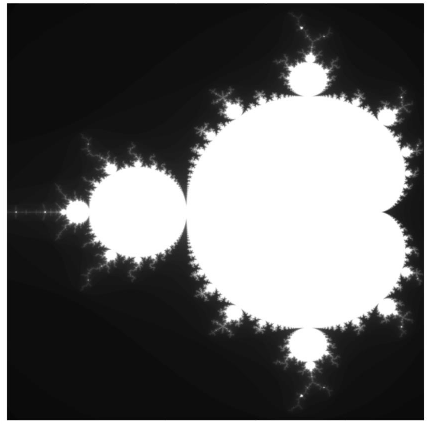
\includegraphics[width=3.5cm]{images/mandelbrot}
  \end{center}
  
\end{frame}

%%%%%%%%%%%%%%%%%%%%%%%%%%%%%%%%%%%%%%%%%%%%%%%%%%%%%%%%%%%%%%%%%%%%%%%% 
%%%%%%%%%%%%%%%%%%%%%%%%%%%%%%%%%%%%%%%%%%%%%%%%%%%%%%%%%%%%%%%%%%%%%%%% 
\begin{frame}[fragile=singleslide]
  \frametitle{Hands-On 3 : Mandelbrot set}

  {\Large \textcolor{darkgreen}{\textbf{Proposed activity:}}\\ \textbf{refactor this computing loop into a C++ Kokkos functor class}}
  \begin{itemize}
  \item See \textcolor{blue}{kokkos basic version} from \texttt{code/handson/3/mandelbrot\_kokkos/kokkos\_basic} (already a bit refactored to ease the job)
  \end{itemize}
  %
  \begin{enumerate}
  \item we added a file \textcolor{blue}{\texttt{kokkos\_shared.h}}: \texttt{std::vector} replaced by a \texttt{Kokkos::View}
  \item \textcolor{orange}{\textbf{TODO:}} fill TODOs in \texttt{mandelbrot.h} containing the definition of the c++ mandelbrot kokkos functor.\\
    \textbf{Notice:} the global constants have disappeared, they are now part of the functor context.
  \item \textcolor{orange}{\textbf{TODO:}} refactor \texttt{main.cpp} (change the TODO)
    \begin{itemize}
    \item Modify data allocation (from \texttt{std::vector} to \texttt{Kokkos::View}); we have now arrays: \texttt{image} and \texttt{imageHost} (mirror)
    \item Copy back results from device to host.
    \end{itemize}
  \end{enumerate}
  
\end{frame}

%%%%%%%%%%%%%%%%%%%%%%%%%%%%%%%%%%%%%%%%%%%%%%%%%%%%%%%%%%%%%%%%%%%%%%%% 
%%%%%%%%%%%%%%%%%%%%%%%%%%%%%%%%%%%%%%%%%%%%%%%%%%%%%%%%%%%%%%%%%%%%%%%% 
\begin{frame}[fragile=singleslide]
  \frametitle{Hands-On 3 : Mandelbrot set}

  \begin{itemize}
    % \item The provided \texttt{Makefile} is designed to be used with kokkos environment from a modulefile
  \item Use code from directory \texttt{code/handson/3}; it is designed to work with cmake
  \item Build the \textcolor{blue}{\texttt{kokkos\_basic}} version
  \item \textcolor{violet}{\textbf{OpenMP}}
    \begin{itemize}
    %\item \texttt{module use /pwrwork/workshops/patc-201701/kokkos/modulefiles}
    %\item \texttt{module load kokkos/openmp\_gnu485\_dev}
    \item \texttt{mkdir build\_openmp; cd build\_openmp}
    \item \texttt{cmake -DKOKKOS\_ENABLE\_OPENMP=ON ..; make}
    \end{itemize}
  \item \textcolor{violet}{\textbf{Cuda}}
    \begin{itemize}
    %\item \texttt{module use /pwrwork/workshops/patc-201701/kokkos/modulefiles}
    %\item \texttt{module load cuda/8.0 kokkos/cuda80\_gnu485\_dev\_k80}
    \item \texttt{mkdir build\_cuda; cd build\_cuda\_kepler37}
    \item \texttt{export CXX=/full/path/to/nvcc\_wrapper}
    \item \texttt{cmake -DKOKKOS\_ENABLE\_CUDA=ON -DKOKKOS\_ARCH=Kepler37 ..}
    \item you also add \texttt{-DKOKKOS\_ENABLE\_CUDA\_LAMBDA=ON}; you can also build again for architecture Pascal60
    \item \texttt{make}
    \end{itemize}
  \item \textbf{Compare performance} for a large Mandelbrot set $8192\times 8192$ : OpenMP versus Cuda
  \end{itemize}

\end{frame}
  
%%%%%%%%%%%%%%%%%%%%%%%%%%%%%%%%%%%%%%%%%%%%%%%%%%%%%%%%%%%%%%%%%%%%%%%% 
%%%%%%%%%%%%%%%%%%%%%%%%%%%%%%%%%%%%%%%%%%%%%%%%%%%%%%%%%%%%%%%%%%%%%%%% 
\begin{frame}[fragile=singleslide]
  \frametitle{Hands-On 3 : Mandelbrot set}

  \begin{itemize}
  \item {\bf Additionnal:} revisit this simple example using a \textcolor{blue}{\bf multidimensional range policy} to launch the Mandelbrot functor:
  \end{itemize}
  \begin{minted}{c++}
    Kokkos::Experimental::MDRangePolicy< Kokkos::Experimental::Rank<2> ,
                                         Kokkos::IndexType<int> >;
  \end{minted}
  \begin{itemize}
  \item \textcolor{orange}{\textbf{TODO:}} fill TODOs in \texttt{mandelbrot.h} and \texttt{main.cpp} in directory \texttt{mandelbrot\_kokkos/kokkos\_mdrange}
  \item \textcolor{red}{\bf This way avoids the use of linearized indexes.}
  \end{itemize}

\end{frame}

%%%%%%%%%%%%%%%%%%%%%%%%%%%%%%%%%%%%%%%%%%%%%%%%%%%%%%%%%%%%%%%%%%%%%%%% 
%%%%%%%%%%%%%%%%%%%%%%%%%%%%%%%%%%%%%%%%%%%%%%%%%%%%%%%%%%%%%%%%%%%%%%%% 
\begin{frame}[fragile=singleslide]
  \frametitle{Hands-On 3 : Mandelbrot set}

  \begin{itemize}
  \item Pipelined version of Mandelbrot is not currently fully functional; it requires a small patch applied to \texttt{Kokkos} for \texttt{cudaStreams};\\
    see \myurl{https://github.com/kokkos/kokkos/issues/532}
  \item Understand what is pipelined version of Mandelbrot see:
    {\scriptsize \myurl{http://on-demand.gputechconf.com/gtc/2015/webinar/openacc-course/advanced-openacc-techniques.pdf}}\\
    It basically consists in overlapping GPU computations with CPU/GPU memory transfert.
  \item See explanations given during training
  \end{itemize}

\end{frame}
